\subsection{DFA accepting a 001 substring}

\renewcommand{\CURPATH}{synth/DFA}

\begin{lstlisting}
This example shows how to design a finite automaton E_2 to recognize the regular
language of all strings that contain the string 001 as a substring. For example,
0010, 1001, 001, and 11111110011111 are all in the language, but 11 and 0000
are not. How would you recognize this language if you were pretending to
be E_2?
\end{lstlisting}
( M.Sipser --- Introduction to the Theory of Computation, 2ed, p43, Example 1.21. )

\lstinputlisting[style=custompy]{\CURPATH/1.py}

\begin{figure}[H]
\centering
%\frame{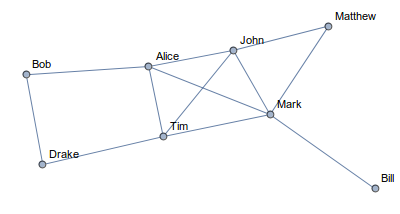
\includegraphics[scale=0.7]{\CURPATH/graph1.png}}
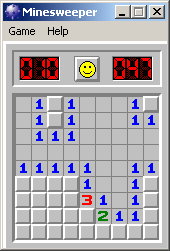
\includegraphics[scale=0.7]{\CURPATH/1.png}
\end{figure}

